\documentclass[tikz]{standalone}

\begin{document}
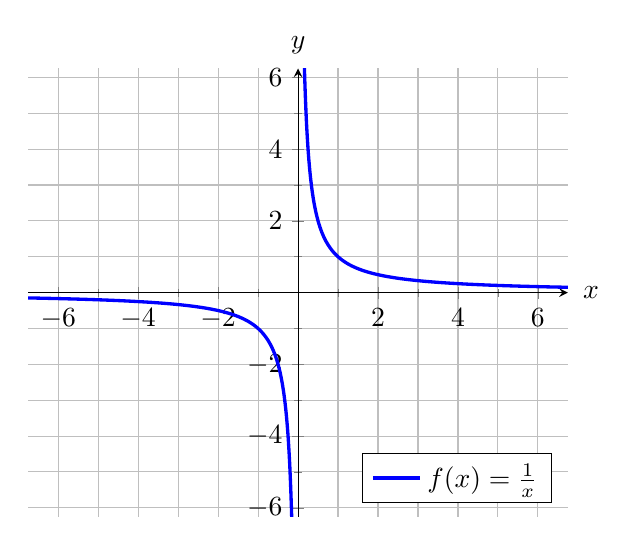
\begin{tikzpicture}
    \begin{axis}[%
        xlabel=$x$, ylabel=$y$, legend pos=south east,
        grid=both, xmin=-6.75, xmax=6.75, ymin=-6.25, ymax=6.25,
        axis lines = middle,
        minor x tick num=1, minor y tick num=1,
        xlabel style = {at={(axis description cs:1.01,0.5)},anchor=west},
        ylabel style = {at={(axis description cs:0.5,1.01)},anchor=south},
    ]
    \addplot[blue, very thick, smooth, samples=200, domain=-10:-0.1] plot {1/x};
    \addplot[blue, very thick, smooth, samples=200, domain=0.1:10] plot {1/x};
    \legend{$f(x)=\frac{1}{x}$}
    \end{axis}
\end{tikzpicture}
\end{document}
